\documentclass[a4paper,11pt]{article}

\usepackage{mlsubmit}

\begin{document}

\initmlsubmision{2} % assignment number
{Divyaksh Shukla}   % your name
{231110603}	% your roll number

\date{November 8, 2023}

\begin{mlsolution}

\begin{itemize}
    \item This is solved by taking the cluster which has its mean closest to the test point $x_n$ $$ \arg\min_{k}||x_n-\mu_k||^{2} $$
    \item If we assume the test point to be closest to a cluster mean, denoted by $\mu_{k}$ then we can get the update equation for $\mu_{k}$ by taking derivative of $\mathcal{L}$ w.r.t. $\mu_{k}$ $$ \frac{\partial \mathcal{L}}{\partial \mu_{k}} = -2||x_{n} - \mu_{k}|| $$ Which can be put into the update equation as \begin{equation}
        \mu_{k} = \mu_{k} + \eta ||x_{n} - \mu_{k}||
        \label{eq:k-means-sgd-update}
    \end{equation}
    \item In \ref{eq:k-means-sgd-update} we have taken all constants to be part of the step-size $\eta$. A good choice of $\eta$ would be a small value that decreases monotonically as the steps progress. By taking a small step size the cluster means will slowly progress towards the expected means and remain unaffected by noisy input datapoints.
\end{itemize}

% A vector symbol $\vb$, a symbol in blackboard font $\bR$, a symbol in calligraphic font $\cA$, \red{some} \green{colored} \blue{text}


\end{mlsolution}

\begin{mlsolution} 

As $z_n \in \mathop{\mathbb{R}}$ is a linear transformation of $\vx_n$ and $\vw$ we can write:
$$z_n=\vw^T\vx_n$$
We need to minimise distance between each projected point $z_n$ and its cluster mean, say $\bc{\mu_-, \mu_+}$ and maximize distance between the projected means.
\begin{equation}
    \max \abs{\mu_- - \mu_+}
\end{equation}
\begin{equation}
    \min \sum_{z_n:y_n=+1}{\abs{z_n - \mu_+}} + \sum_{z_n:y_n=-1}{\abs{z_n - \mu_-}}
\end{equation}

\noindent Thus the objective function is:
\begin{equation}
    J = \max\left[ \abs{\mu_- - \mu_+} - \sum_{z_n:y_n=+1}{\abs{z_n - \mu_+}} - \sum_{z_n:y_n=-1}{\abs{z_n - \mu_-}} \right]
\end{equation}
as all values are in $\mathop{\mathbb{R}}$ taking only simple absolute distance suffices.


\end{mlsolution}

\begin{mlsolution}

\noindent Let us take $\vS^{\prime}=\frac{1}{N}\vX\vX^T$. Equation \ref{eq:S-prime-eigenequation} represents the equation to calculate eigenvalue $\lambda^{\prime}$ and eigenvector $\vv$ of $\vS^{\prime}$
\begin{equation}
    \vS^{\prime} \vv = \lambda^{\prime} \vv
    \label{eq:S-prime-eigenequation}
\end{equation}

\noindent Now if we take the value of $\vS^{\prime}$ and pre-multiply with $\vX^T$ and readjust the values we get:

\begin{align}
    \frac{1}{N}\vX\vX^T\vv &= \lambda^{\prime} \vv \\
    \red{\frac{1}{N}\vX^T\vX}\blue{\vX^T\vv} &= \lambda^{\prime} \blue{\vX^T \vv} \label{eq:Eigenvector-semi-final} \\
    \red{\vS} \blue{\vu} &= \lambda^{\prime} \blue{\vu}
    \label{eq:Eigenvector-final}
\end{align}

\noindent Thus the eigenvalue remains the same in both forms, only the eigenvectors change, which can be seen in blue from Equation \ref{eq:Eigenvector-semi-final} and \ref{eq:Eigenvector-final}. By computing eigenvectors this way we can reduce the complexity of calculating eigenvalues for a $D\times D$ matrix to $N\times N$ matrix, which is feasible in this case as $D<N$.

\end{mlsolution}

\begin{mlsolution}

\section*{Part 1}
    In practical scenarios the input data need not be a part of a single distribution. By modelling with latent input variables $\vz_n$ we can leverage the fact that the input is coming from different distributions and so we can apply a combination of K different linear models to predict $y_n$ from $\vx_n$. This can also be useful in outlier detection as the outlier input point will be a part of its own cluster.
\section*{Part 2}
    The latent variable model is defined in Equation \ref{eq:basic-lvm-model}
    \begin{equation}
        \label{eq:basic-lvm-model}
        p(\vz_n|\vx_n,\Theta) = \frac{p(\vz_n|\Theta)p(\vx_n|\vz_n,\Theta)}{p(\vx_n|\Theta)}
    \end{equation}
    Upon applying the variables and distributions from the question we get Equation \ref{eq:my-lvm-model}. Now that we only have to take MLE solution we can reduce the same to \ref{eq:my-lvm-mle-model}
    \begin{align}
        p(z_n=k|y_n,\Theta) &= \frac{p(z_n=k|\Theta)p(y_n|z_n=k,\Theta)}{p(y_n|\Theta)} \label{eq:my-lvm-model} \\
        &= p(z_n=k|\Theta)p(y_n|z_n=k,\Theta) \label{eq:my-lvm-mle-model}
    \end{align}
    where:
    \begin{align}
        p(z_n=k|\Theta) &= \pi_k \\
        p(y_n|z_n=k,\Theta) &= \mathop{\mathcal{N}}(w^T_{z_n}x_n, \beta^{-1})
    \end{align}
    Taking the log of equation \ref{eq:my-lvm-mle-model} with the provided distributions we get:
    \begin{align}
        \log{p(z_n=k|y_n,\Theta)} &= \log{\pi_k} + \log{\mathop{\mathcal{N}}(w^T_{z_n}x_n, \beta^{-1})}
    \end{align}
    \textbf{ALT-OPT ALGORITHM}

    \noindent Step 1: Find the best $z_n$
    \begin{align}
        \hat{z_n} &= \argmax_{k=1,2,...,k} \log{\pi_k} + \log{\mathop{\mathcal{N}}(w^T_{z_n}x_n, \beta^{-1})}\\
        &= \argmax_{k=1,2,...,k} \log{\pi_k} + \frac{\beta}{2}\br{y_n-w^T_{z_n}x_n}
    \end{align}
    Step 2: re-estimate the parameters
    \begin{align}
        \pi_k &= \frac{N_k}{N}\\
        w_k &= (X^T_kX_k)^{-1}X^T_ky_k
    \end{align}
    Where $N_k$ is the number of points in cluster $k$
    
\end{mlsolution}
	
\begin{mlsolution}

    \section{Kernel Ridge Regression}
        \subsection{Regularized Kernel Ridge Regression}
            I calculated the output for the test-point by using Equation \ref{eq:kernel-ridge-1}.
            \begin{equation}
                \label{eq:kernel-ridge-1}
                \vY^*=\vK^*(\vK-\lambda \vI_N)^{-1}\vY
            \end{equation}
            where $\vK*$ and $\vK$ are the kernel matrices: $\vK^*=k(x*,x_n)$, $\vK=k(x_m,x_n)$ and $k(x_m,x_n) = exp\left( -\gamma\abs{\abs{x_n - x_m}}^2 \right)$ is the rbf kernel function.
            The RMSE value is calculated using: $$\sqrt{\frac{1}{N}||y_{true} - y_{pred}|| ^2}$$
            \begin{figure}[h]
                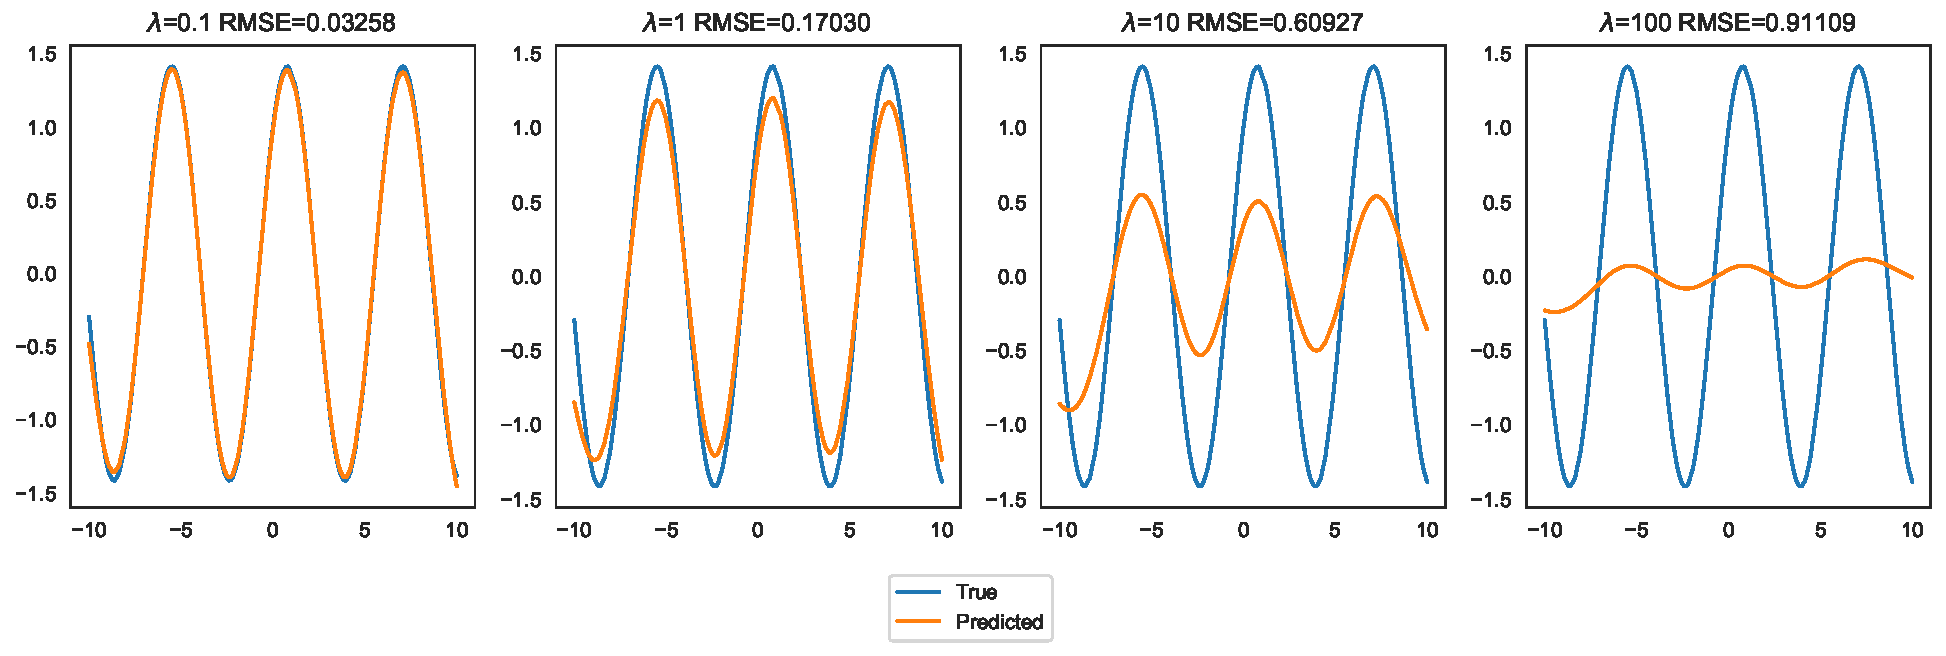
\includegraphics[width=\textwidth]{images/kernel-ridge-regression.pdf}
                \caption{Kernel ridge regression with different regularizations}
                \label{fig:kernel-rdge-regression}
            \end{figure}
            
            From Figure \ref{fig:kernel-rdge-regression} we can see that as we increase the regularization hyperparameter $\lambda$ from $0.1$ to $100$ we see that the predictions are not able to accurately predict the noiseless y-values. Adding regularization makes the model resistant to noise and improves test-accuray, but in this case the y-values in test data are noiseless so it is better to overfit the model to reduce RMSE value.
        \subsection{Landmark Kernel Ridge Regression}
        Here I randomly chose $2$, $5$, $20$, $50$ and $100$ landmark points from train data and ran the same kernel ridge regression code on the test data. From Figure \ref{fig:landmark-kernel-rdge-regression} we can see that as the number of Landmark points increases the regression model starts to predict the model in a better way, the RMSE reduces.
        \begin{figure}[h]
            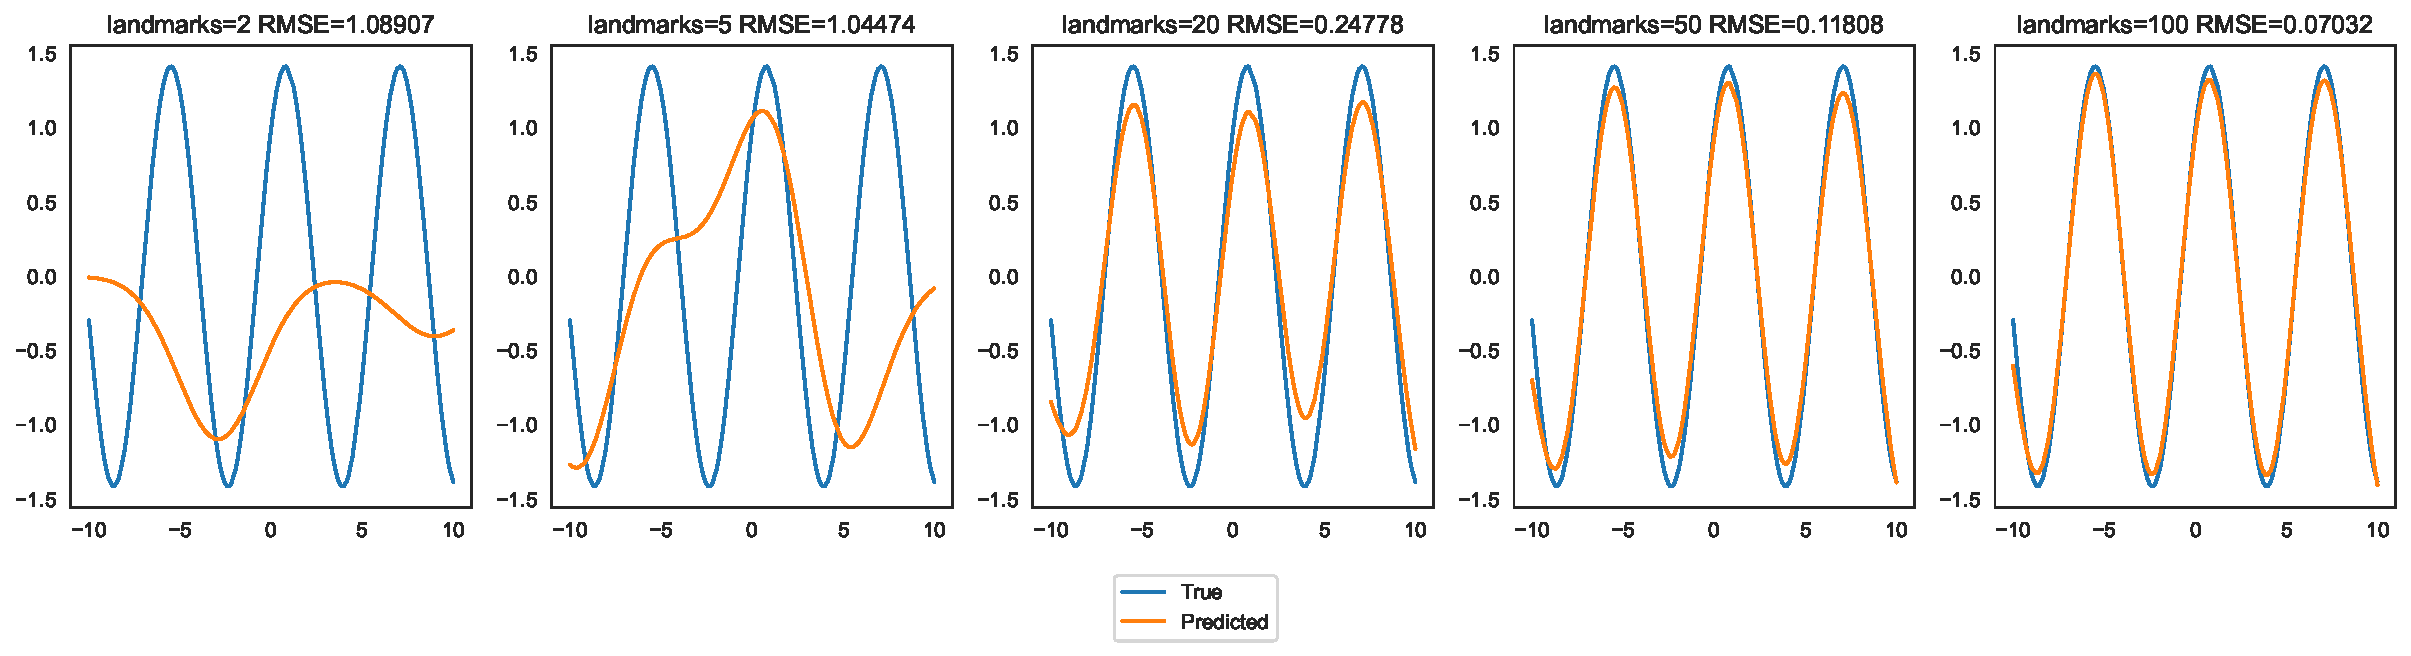
\includegraphics[width=\textwidth]{images/landmark-kernel-ridge-regression.pdf}
            \caption{Landmark kernel ridge regression with different number of landmark points}
            \label{fig:landmark-kernel-rdge-regression}
        \end{figure}

    \section{K-Means Clustering}

        In Figure \ref{fig:k-means-initial-plot} we see that the data is circular and there are 2 intuitive clusters that are possible. So I calculated the radius of each point by applying \ref{eq:angle-calc} and \ref{eq:radius-calc} and then projecting all the points on 1-dimension to get Figure \ref{fig:k-means-with-radius-projection} and applying k-means on the projected data to obtain Figure \ref{fig:k-means-clustered-with-radius-projection}
        \begin{figure}[h]
            \centering
            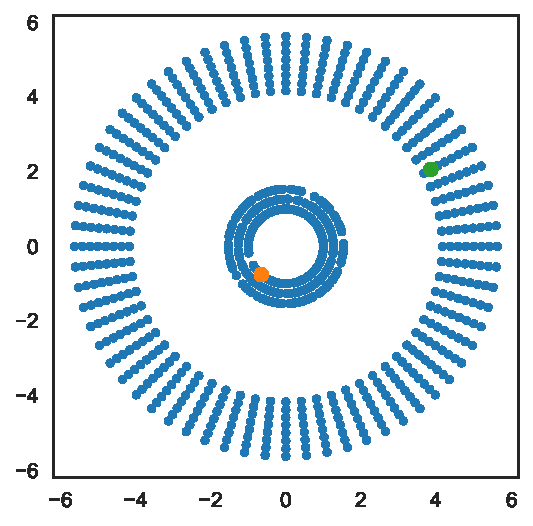
\includegraphics[width=.3\textwidth]{images/k-means-initial-plot.pdf}
            \caption{Scatter plot of data with initial centers highlighted}
            \label{fig:k-means-initial-plot}
        \end{figure}

        \begin{equation}
            \label{eq:angle-calc}
            \theta = tan^{-1}\left( \frac{y}{x} \right)
        \end{equation}
        \begin{equation}
            \label{eq:radius-calc}
            r = \frac{x}{cos(\theta)}
        \end{equation}

        \begin{figure}[h]
            \centering
            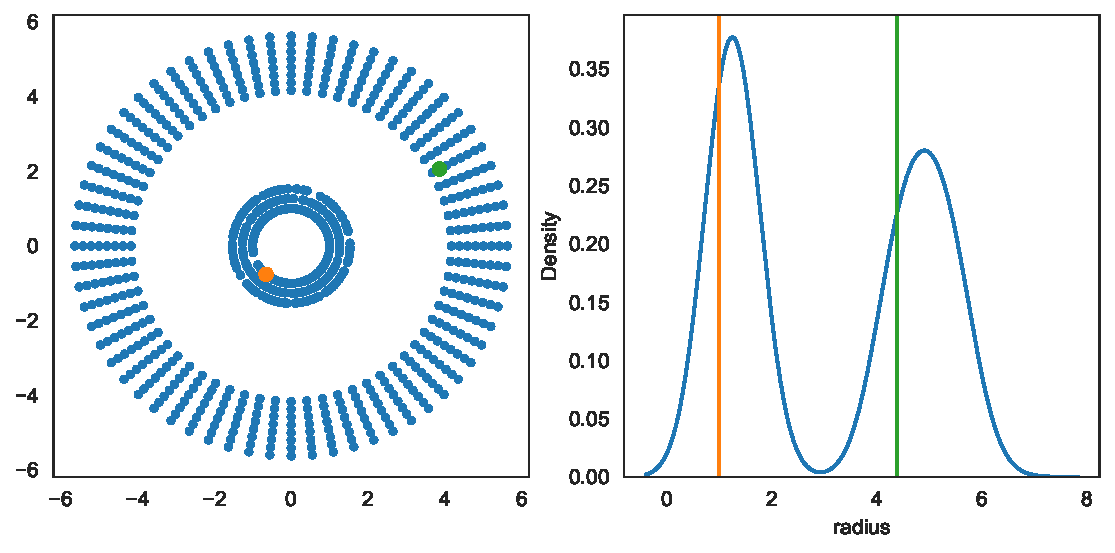
\includegraphics[width=.5\textwidth]{images/k-means-with-radius-projection.pdf}
            \caption{Projecting data points into 1-dimension by taking radius of points from origin. Also highlighting the inital centers}
            \label{fig:k-means-with-radius-projection}
        \end{figure}

        \begin{figure}[h]
            \centering
            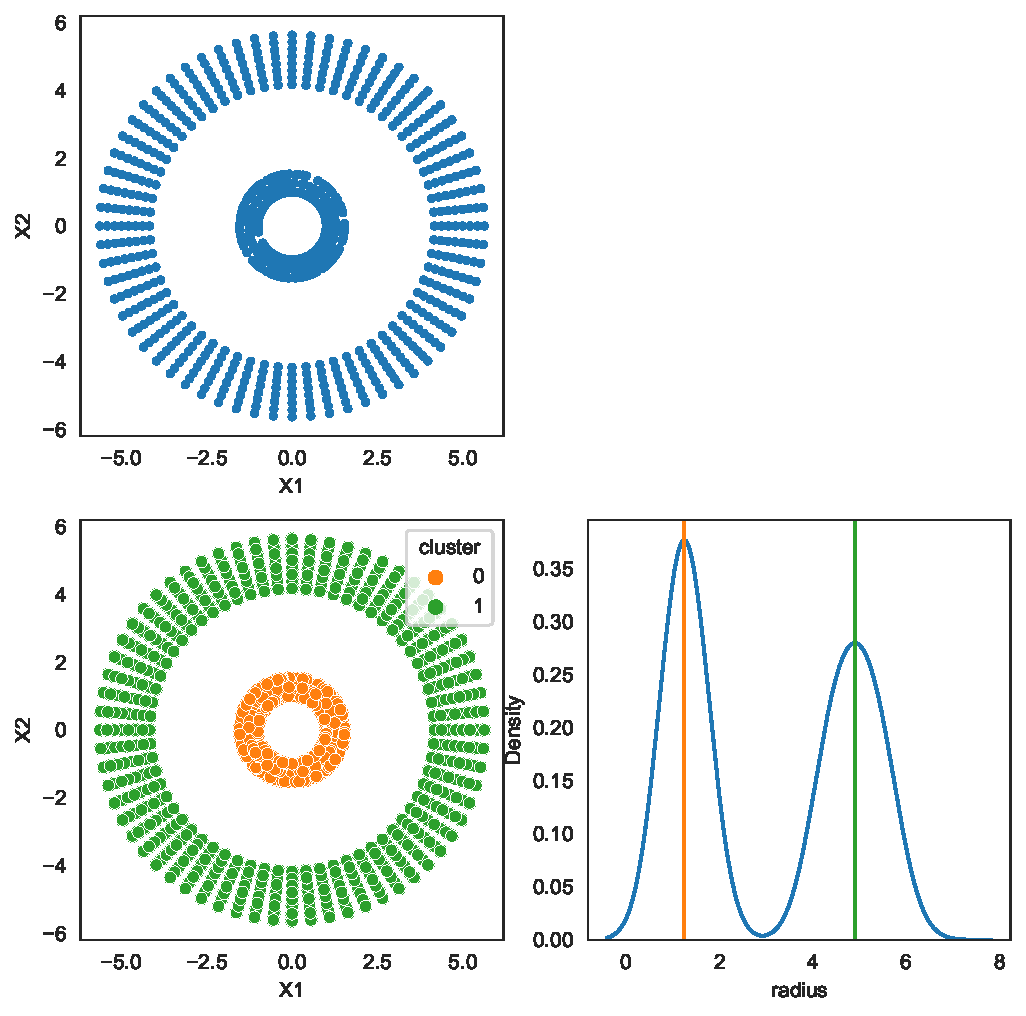
\includegraphics[width=.5\textwidth]{images/k-means-clustered-with-radius-projection.pdf}
            \caption{Clustering the data points based on radius and showing the position of the cluster centers on the 1-dimensional plot.}
            \label{fig:k-means-clustered-with-radius-projection}
        \end{figure}

        Next I chose $1$ landmark point randomly and added another feature based on RBF kernel function. Then I ran a k-means prediction algorithm which led to the good and bad clustering. Figure \ref{fig:k-means-landmark} shows all the clustered plots.

        \begin{figure}[h]
            \centering
            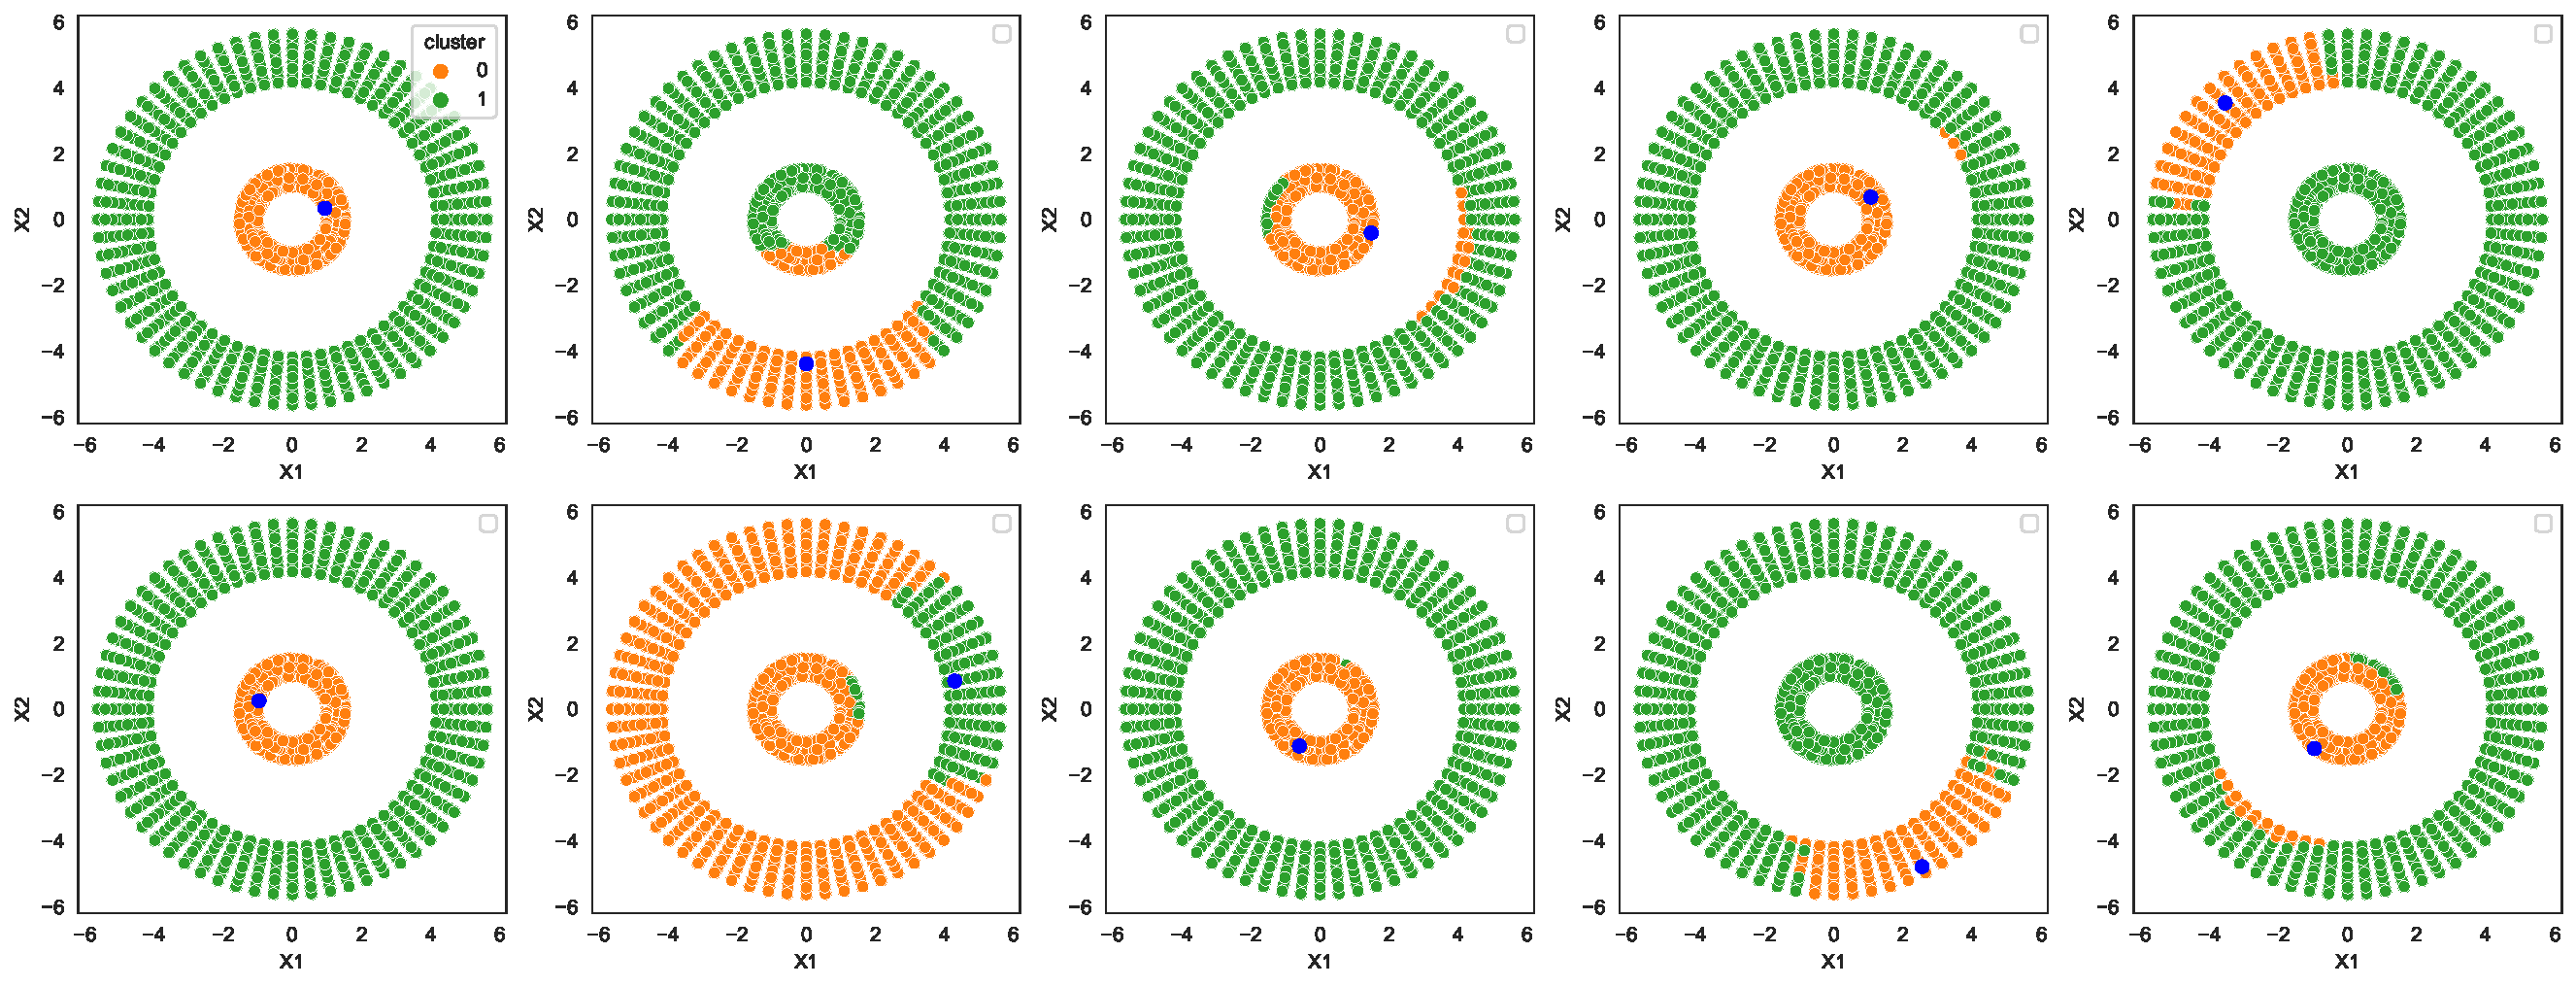
\includegraphics[width=\textwidth]{images/k-means-landmark.pdf}
            \caption{Applying k-means with 1 training landmark point.}
            \label{fig:k-means-landmark}
        \end{figure}

    \section{PCA and TSNE}
        \begin{figure}[h]
            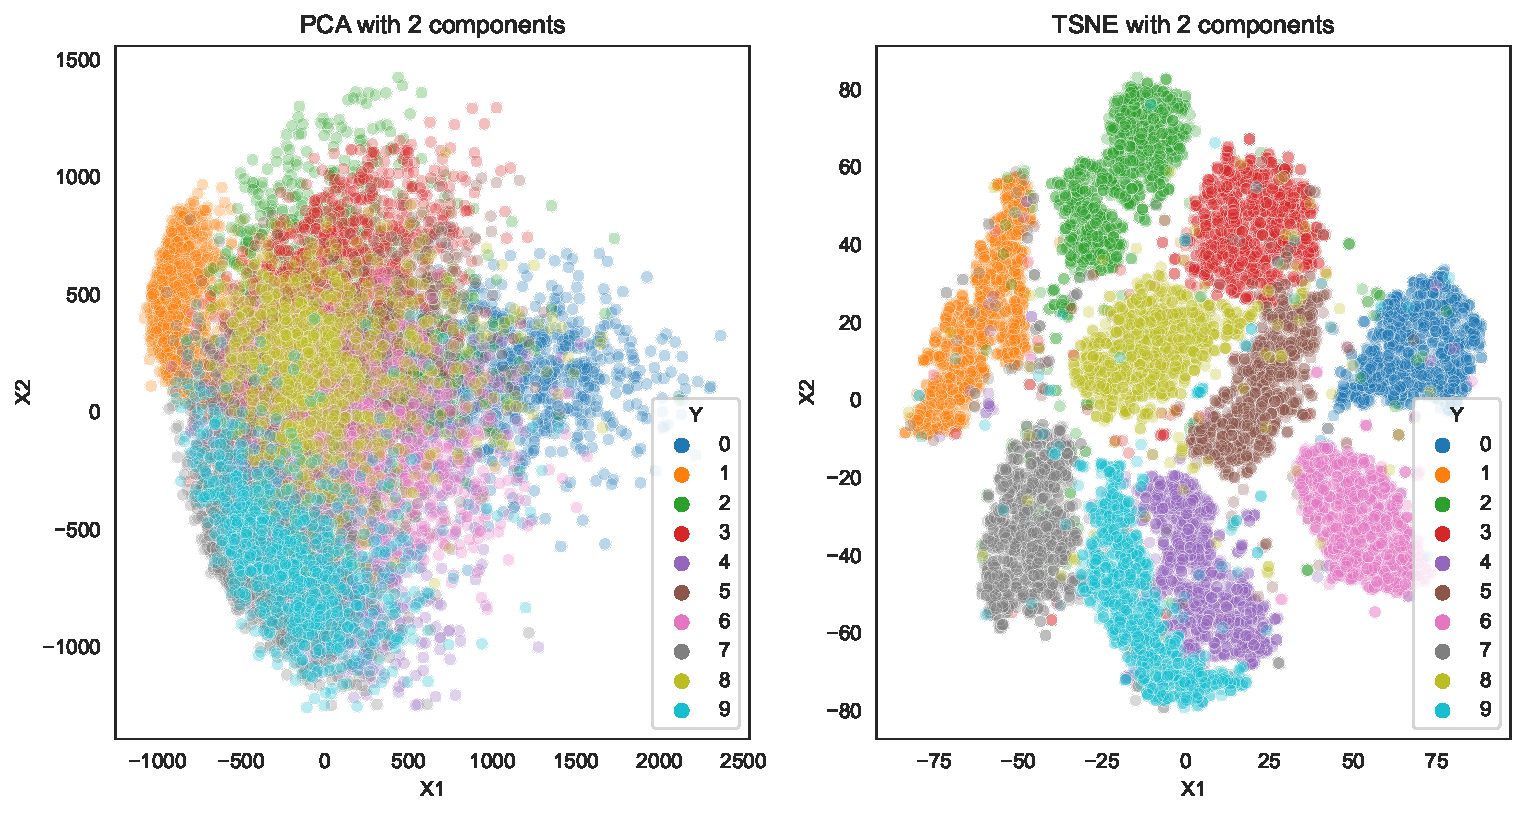
\includegraphics[width=\textwidth]{images/pca-tsne.pdf}
            \caption{2-Dimensional PCA and TSNE plots of MNIST}
            \label{fig:pca-tsne}
        \end{figure}
        TSNE is able to make clusters which are naturally observable on 2 dimensions in a better way compared to PCA. In PCA, we can see significant overlap and mixing of points from different clusters. Thus, TSNE is a better projection technique to visualize high-dimensional data.

\end{mlsolution}


\end{document}
